\documentclass[border=6pt]{standalone}
\usepackage{tikz}
\usetikzlibrary{arrows.meta,positioning,calc}
\usepackage{helvet}
\renewcommand{\familydefault}{\sfdefault}

\begin{document}
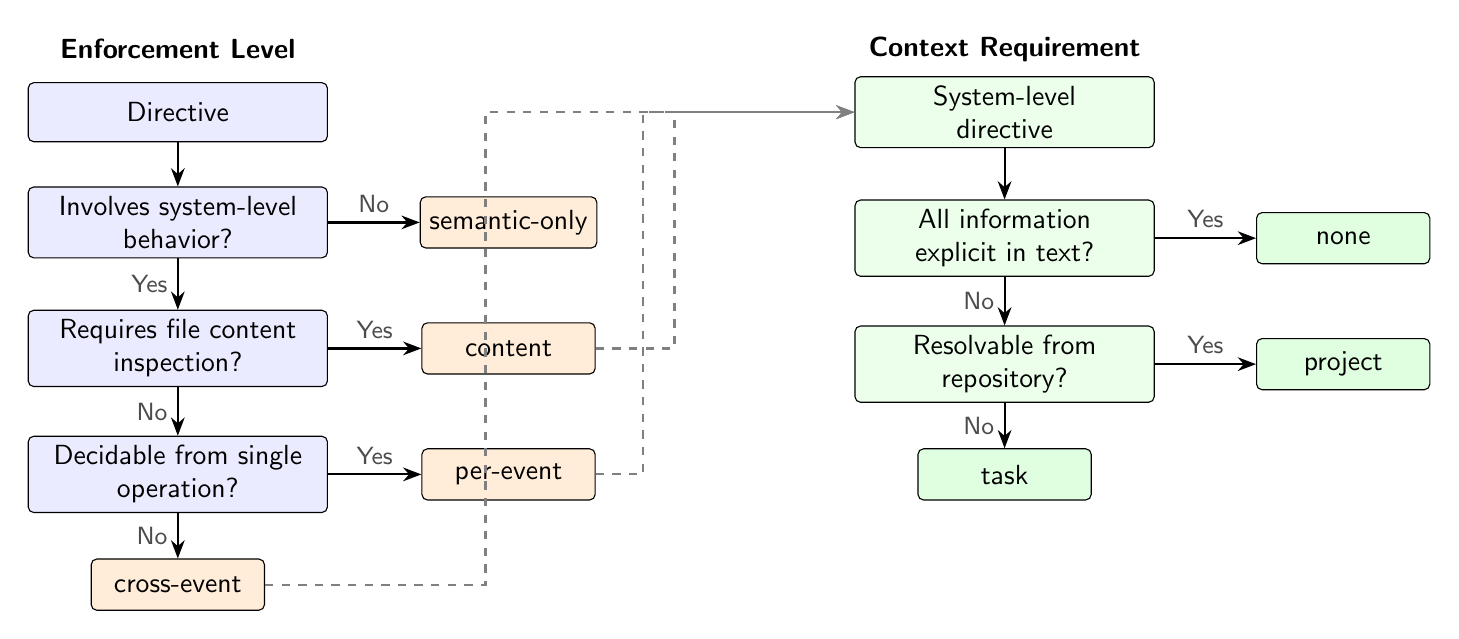
\begin{tikzpicture}[
  >=Stealth,
  decision/.style={draw, rounded corners=2pt, minimum height=0.75cm,
              minimum width=3.8cm, align=center, font=\normalsize,
              fill=blue!8},
  outcome/.style={draw, rounded corners=2pt, minimum height=0.65cm,
              minimum width=2.2cm, align=center, font=\normalsize,
              fill=orange!15},
  arr/.style={->, thick},
  lbl/.style={font=\small, text=black!70},
  title/.style={font=\normalsize\bfseries},
]

% === Left: Enforcement level waterfall ===
\node[title] at (0,5.8) {Enforcement Level};

\node[decision] (start) at (0,5.0) {Directive};

\node[decision] (q1) at (0,3.6) {Involves system-level\\behavior?};
\node[outcome] (sem) at (4.2,3.6) {semantic-only};

\node[decision] (q2) at (0,2.0) {Requires file content\\inspection?};
\node[outcome] (cont) at (4.2,2.0) {content};

\node[decision] (q3) at (0,0.4) {Decidable from single\\operation?};
\node[outcome] (per) at (4.2,0.4) {per-event};

\node[outcome] (cross) at (0,-1.0) {cross-event};

% Arrows
\draw[arr] (start) -- (q1);
\draw[arr] (q1) -- node[above, lbl] {No} (sem);
\draw[arr] (q1) -- node[left, lbl] {Yes} (q2);
\draw[arr] (q2) -- node[above, lbl] {Yes} (cont);
\draw[arr] (q2) -- node[left, lbl] {No} (q3);
\draw[arr] (q3) -- node[above, lbl] {Yes} (per);
\draw[arr] (q3) -- node[left, lbl] {No} (cross);

% === Right: Context requirement waterfall ===
\node[title] at (10.5,5.8) {Context Requirement};

\node[decision, fill=green!8] (start2) at (10.5,5.0) {System-level\\directive};

\node[decision, fill=green!8] (cq1) at (10.5,3.4) {All information\\explicit in text?};
\node[outcome, fill=green!12] (none) at (14.8,3.4) {none};

\node[decision, fill=green!8] (cq2) at (10.5,1.8) {Resolvable from\\repository?};
\node[outcome, fill=green!12] (proj) at (14.8,1.8) {project};

\node[outcome, fill=green!12] (task) at (10.5,0.4) {task};

% Arrows
\draw[arr] (start2) -- (cq1);
\draw[arr] (cq1) -- node[above, lbl] {Yes} (none);
\draw[arr] (cq1) -- node[left, lbl] {No} (cq2);
\draw[arr] (cq2) -- node[above, lbl] {Yes} (proj);
\draw[arr] (cq2) -- node[left, lbl] {No} (task);

% Connecting arrow from left to right
\draw[arr, dashed, gray] (cont.east) -- ++(1.0,0) |- (start2.west);
\draw[arr, dashed, gray] (per.east) -- ++(0.6,0) |- (start2.west);
\draw[arr, dashed, gray] (cross.east) -- ++(2.8,0) |- (start2.west);

\end{tikzpicture}
\end{document}
